\chapter{Экспериментальная часть и исследовательский вклад}

\section{Сравнительный анализ моделей нейронных сетей для автоматизированного решения CAPTCHA в текстовом формате}

\textbf{Современная реализация текстовых CAPTCHA}

Современные текстовые CAPTCHA обычно состоят из букв и цифр. Зачастую 
используются символы латинского алфавита (как прописные, так и строчные) и цифры 
от 0 до 9. Но обычно реализации исключают символы, которые могут быть легко 
перепутаны, например, буквы <<O>> и цифру <<0>>, буквы <<I>> и <<l>> и тому 
подобное. Рекомендуемый набор символов в генераторах на некоторых CRM платформах 
выглядит следующим образом: ABCDEFGHJKLMNPQRSTWXYZ23456789~\cite{Bitrix}.

Длина последовательности символов в CAPTCHA обычно составляет от 4 до 8 символов, 
что обеспечивает баланс между удобством для пользователя и безопасностью, однако 
конкретная длина может варьироваться в зависимости от требований системы 
безопасности.

Для усложнения автоматического распознавания текстовые CAPTCHA подвергаются 
различным искажениям:
\begin{enumerate}
    \item геометрические искажения: символы могут быть искажены, повернуты или 
    наклонены, что затрудняет их распознавание автоматическими системами~
    \cite{BrightData};
    \item перекрытие символов: символы могут быть расположены близко друг к 
    другу или даже перекрываться, что усложняет их сегментацию и последующее 
    распознавание~\cite{Proglib};
    \item добавление шума: на изображение могут быть добавлены различные шумы, 
    такие как линии, точки или круги, чтобы затруднить распознавание символов;
    \item сложные фоны: использование фонов с различными цветами или узорами, 
    что делает выделение символов более сложным~\cite{NVJournal};
    \item нелинейные искажения: применение нелинейных трансформаций к символам, 
    что делает их форму менее предсказуемой для автоматических систем 
    распознавания~\cite{Simai}.
\end{enumerate}

Эти методы направлены на повышение сложности автоматического распознавания 
CAPTCHA, сохраняя при этом относительную легкость распознавания для человека. 

\textbf{Подготовка датасета с изображениями и выбор модели нейронной сети}

Качество используемого датасета оказывает существенное влияние на итоговую 
точность работы модели. Для эффективного обучения необходимо, чтобы набор данных 
соответствовал следующим требованиям:

\begin{enumerate}
    \item достаточное количество изображений для каждого символа, что 
    обеспечивает статистическую устойчивость модели;
    \item разнообразие данных, включающее:
    \begin{enumerate}
        \item различные углы наклона символов;
        \item вариативность написания символов и их искажения;
        \item наличие побочных визуальных элементов, создающих препятствия для 
        распознавания;
        \item использование различных шрифтов.
    \end{enumerate}
    \item переменная длина последовательностей символов, что позволяет модели 
    адаптироваться к разным формам CAPTCHA.
\end{enumerate}

Включение указанных факторов способствует обучению модели на более широком 
спектре признаков, что, в свою очередь, повышает её способность к обобщению на 
ранее невидимых данных.

Для распознавания текста с переменной длиной последовательности в задачах CAPTCHA 
наиболее часто применяются следующие архитектуры нейронных сетей:

\begin{enumerate}
    \item оптическое распознавание символов (OCR);
    \item рекуррентные сверточные нейронные сети (CRNN);
    \item архитектуры последовательного обучения (Seq-to-Seq).
\end{enumerate}

С целью выбора наиболее эффективной модели были реализованы и протестированы все 
указанные подходы, после чего была выбрана архитектура, обеспечивающая наилучшую 
точность предсказаний.

Для обучения моделей был сформирован датасет из 100 000 изображений CAPTCHA, 
содержащих случайные последовательности символов длиной от 4 до 7. Такой объем 
данных позволяет добиться высокой обобщающей способности модели и снизить 
вероятность переобучения.

\textbf{Оптическое распознавание символов (OCR Tesseract)}

Изначально предполагалась реализация модели с использованием OCR, поскольку такие 
системы изначально разрабатывались для задач оптического распознавания текста. В 
качестве конкретной модели был выбран Tesseract.

Tesseract является одной из наиболее популярных систем OCR с открытым исходным 
кодом. Tesseract поддерживает более 100 языков, включая сложные письменности~
\cite{Klippa}. В версии 4.0 в модель была интегрирована нейронная сеть на основе 
долговременной краткосрочной памяти (LSTM), что позволило существенно повысить 
точность распознавания, особенно при обработке сложных шрифтов и рукописного 
текста~\cite{GitTesseract}.

Для решения поставленной задачи предполагалось использовать предобученную модель 
Tesseract и дообучить её на специализированном датасете, содержащем изображения 
CAPTCHA с характерными искажениями. Однако в ходе экспериментов было установлено, 
что точность распознавания последовательностей символов целиком составляла 0\%, а 
точность для отдельных символов оказалась крайне низкой. Это связано с тем, что 
архитектура Tesseract недостаточно устойчива к искажениям, характерным для 
CAPTCHA, таким как деформация символов, наложение шумов и изменение углов наклона
~\cite{TrainTesseract}.

Таким образом, было принято решение отказаться от использования Tesseract в 
пользу более адаптированных к данной задаче моделей, таких как сверточные 
рекуррентные нейронные сети (CRNN) или модели последовательного обучения 
(Seq-to-Seq), обладающие высокой устойчивостью к вариативности и искажениям, 
характерным для CAPTCHA.

\textbf{Рекуррентные сверточные нейронные сети (CRNN)}

Сверточно-рекуррентные нейронные сети (CRNN) представляют собой гибридную 
архитектуру, сочетающую в себе возможности сверточных нейронных сетей (CNN) и 
рекуррентных нейронных сетей (RNN). Данный подход используется в задачах, 
связанных с обработкой последовательных данных, таких как распознавание текста, 
речь и видео~\cite{CRNNHabr}.

Основное преимущество CRNN заключается в способности CNN-части извлекать 
пространственные признаки из изображений, тогда как RNN-часть позволяет учитывать 
временные зависимости между последовательными фрагментами данных~\cite{CRNNBook}.

Разработанная модель CRNN для распознавания CAPTCHA включает в себя три ключевых 
блока:
\begin{enumerate}
    \item сверточный блок (CNN): предназначен для выделения признаков из 
    изображений CAPTCHA. Включает в себя три последовательных сверточных слоя, а 
    также методы нормализации и уменьшения размерности признакового пространства;
    \item рекуррентный блок (RNN): использует двунаправленные слои GRU, 
    позволяющие модели учитывать зависимость между последовательными символами в 
    CAPTCHA;
    \item выходной слой: полносвязный, который выполняет классификацию каждого 
    символа в последовательности.
\end{enumerate}

В приложении~\ref{code:crnn} представлена реализация CRNN-модели на языке Python 
с использованием библиотеки TensorFlow/Keras:

В данной архитектуре применяются слои Dropout для регуляризации, также 
используется l2-регуляризация, BatchNormalization для ускорения обучения и 
повышения устойчивости модели, а также функция softmax для предсказания классов 
символов.

После обучения данной модели результаты оказались превосходящими показатели OCR, 
однако все же не достигли удовлетворительного уровня. В частности, точность 
распознавания всей последовательности символов не превышала 10\%, тогда как 
точность классификации отдельных символов составляла около 70\%.

\textbf{Архитектура последовательного обучения (Seq-to-Seq)}

Модели последовательного преобразования (Seq-to-Seq) широко применяются для 
задач, связанных с обработкой последовательностей переменной длины. Они 
используются в таких областях, как машинный перевод, распознавание речи и анализ 
текстов~\cite{Seq2Seq}. Данные модели основаны на архитектуре энкодера-декодера, 
где первый модуль кодирует входную последовательность в скрытое представление, а 
второй декодирует его в выходную последовательность.

Одним из ключевых элементов Seq2Seq является механизм внимания, который позволяет 
декодеру динамически фокусироваться на различных частях входной 
последовательности при генерации выходных символов~\cite{Seq2SeqBook}. Этот 
подход особенно полезен для распознавания CAPTCHA, так как символы в изображениях 
могут иметь разную ориентацию и степень искажения.

Кодировщик, в данной модели принимает входное изображение CAPTCHA и преобразует 
его в компактное представление. Архитектура кодировщика включает:
\begin{enumerate}
    \item четыре сверточных блока, слои пакетной нормализации и слои подвыборки 
    для понижения размерности входных данных;
    \item глобальный усредненный слой для получения векторного представления 
    изображения;
    \item полносвязный слой для финального представления скрытого состояния;
    \item рекуррентный слой для кодирования последовательности, возвращающий 
    последнее скрытое состояние кодировщика.
\end{enumerate}

Декодировщик выполняет пошаговую генерацию выходной последовательности, используя 
скрытое состояние кодировщика. В архитектуру декодировщика входят:
\begin{enumerate}
    \item входной слой для последовательности токенов;
    \item слой вложения, который преобразует входные токены в векторные 
    представления;
    \item рекуррентный слой, обрабатывающий последовательность с учетом скрытого 
    состояния кодировщика;
    \item механизм внимания, который позволяет декодеру учитывать релевантные 
    части входного изображения;
    \item полносвязный слой с функцией активации softmax для предсказания 
    вероятностей символов.
\end{enumerate}

Полная архитектура модели реализована в TensorFlow/Keras и реализация модели 
приведена в приложении~\ref{code:seq2seq}.

На начальных этапах экспериментов предложенная Seq-to-Seq-модель показала 
наилучшие результаты среди рассмотренных вариантов. В отличие от OCR- и 
CRNN-моделей, данная архитектура смогла достичь более высокой точности 
распознавания последовательностей символов, что обусловлено применением 
механизма внимания. Дальнейшая работа с моделью была сосредоточена на её 
оптимизации и улучшении параметров обучения.

\section{Эксперименты по аудио- и графическим CAPTCHA}

\textbf{Выбор языка программирования и инстументов для разработки}

Для разработки сервиса по автоматизации распознавания CAPTCHA был выбран язык 
программирования Python и библиотека для автоматизации тестирования 
web-приложений Selenium.

Python обладает рядом преимуществ для решения подобных задач:

\begin{enumerate}
    \item простота и читаемость кода: Python легко использовать благодаря 
    лаконичному синтаксису, что ускоряет разработку и упрощает поддержку проекта;
    \item широкая экосистема библиотек: Для работы с CAPTCHA можно использовать 
    специализированные библиотеки, а также сторонние инструменты для машинного 
    обучения;
    \item поддержка скриптового и объектно-ориентированного подхода: Это делает 
    Python гибким для создания как небольших сценариев автоматизации, так и 
    сложных систем.
\end{enumerate}

Selenium выделяется следующими преимуществами среди других инструментов 
автоматизации:

\begin{enumerate}
    \item кросс-браузерная поддержка: Selenium поддерживает тестирование во всех 
    популярных браузерах, таких как Chrome, Firefox, Edge и Safari;
    \item возможности для взаимодействия с динамическими элементами: Selenium 
    может эмулировать действия пользователя, включая ввод текста, клики и работу 
    с выпадающими меню, что полезно для работы с CAPTCHA;
    \item поддержка различных языков программирования: Хотя Python удобен для 
    автоматизации, Selenium можно использовать с Java, C\#, Ruby и другими 
    языками;
    \item интеграция с другими библиотеками и инструментами: Selenium легко 
    интегрируется с фреймворками для тестирования или системами для распознавания 
    изображений.
\end{enumerate}

Audio CAPTCHA представляет собой элемент, встроенный в web-страницу, который 
содержит в себе ссылку на отрезок звуковой дорожки, которая содержит шум и запись 
голоса.

Подобная запись хорошо поддается распознаванию с использованием современных 
библиотек для распознавания речи, одна из которых была использована для решения 
Audio CAPTCHA в данной работе.

В Python существует множество библиотек для распознавания человеческой речи, 
таких как Google Speech Recognition, Pocketsphinx, DeepSpeech и других [7]. 
Среди них была выбрана библиотека SpeechRecognition по следующим причинам:

\begin{enumerate}
    \item удобство использования: Простота в освоении и интеграции благодаря 
    интуитивно понятному API;
    \item поддержка нескольких API: Библиотека предоставляет интерфейсы для 
    работы с несколькими сервисами, включая Google Web Speech API, IBM Watson, 
    Microsoft Azure и другие [8].
    \item кроссплатформенность: SpeechRecognition работает на Windows, macOS и 
    Linux, что обеспечивает гибкость разработки;
    \item встроенные функции обработки звука: Возможность работы с различными 
    форматами аудио, включая wav, и встроенные методы для улучшения качества 
    записи перед отправкой на обработку;
    \item локальная и облачная обработка: Поддержка локальных движков, таких как 
    PocketSphinx, и облачных сервисов, таких как Google Speech API, что делает 
    библиотеку универсальной для различных задач;
    \item открытый исходный код: Это бесплатная библиотека с открытым кодом, что 
    позволяет исследователям и разработчикам адаптировать её под свои нужды.
\end{enumerate}

\textbf{Описание алгоритма работы программы}

Процесс получения аудиофайла, содержащего CAPTCHA, с web-сайта для последующего 
распознавания и отправку готового решения с использованием Selenium можно 
представить как следующую последовательность шагов:

\begin{enumerate}
    \item Инициализация настроек браузера;
    \item Открытие web-страницы, содержащей CAPTCHA;
    \item Переключение на фрейм с чекбоксом CAPTCHA на web-странице и нажатие на 
    чекбокс;
    \item Переключение на фрейм с CAPTCHA в виде картинки или набора картинок и 
    нажатие на кнопку доступа к аудиофайлу;
    \item Переключение на фрейм с аудиозаписью и поиск элемента, который содержит 
    ссылку на аудиозапись;
    \item Создание запроса на получение файла по ссылке;
    \item Передача файла в решатель для последующей обработки;
    \item Вставка результата распознавания в текстовое поле и подтверждение ввода 
    для успешного решения CAPTCHA.
\end{enumerate}

Для создания запроса на получение файла используется встроенный модуль Python -- 
requests.

Блок-схема, иллюстрирующая приведенный алгоритм представлена на рис.~
\ref{fig:audio-solver}.

\begin{figure}[H]
    \centering
    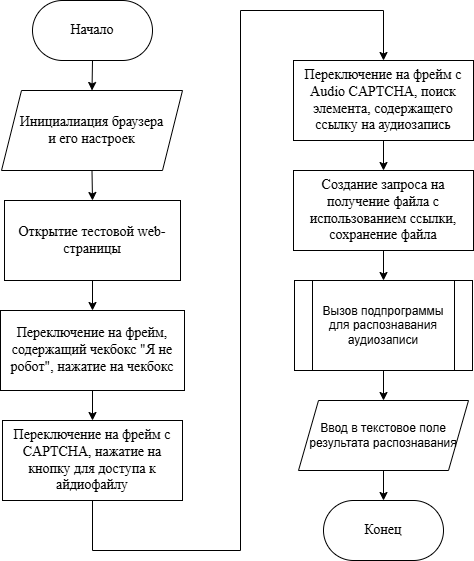
\includegraphics[width=0.6\linewidth]{imgs/audiocaptcha/captcha_solve.png}
    \caption{Блок-схема процесса прохождения Audio CAPTCHA.}
    \label{fig:audio-solver}
\end{figure}

Процесс обработки аудиофайла, полученного с web-страницы можно разделить на 
следующие этапы:

\begin{enumerate}
    \item преобразование полученного аудиофайла в другой формат, который является 
    подходящим для распознавания;
    \item распознавание речи в перекодированном файле;
    \item сохранение полученного результата распознавания для последующей вставки 
    в тектстовое поле.
\end{enumerate}

На первом этапе исходный файл всегда имеет формат mp3, которое не пригодно для 
распознавания с использованием SpeechRecognition, поскольку данный формат 
использует сжатие с потерями, поэтому исходный файл необходимо перекодировать в 
формат wav. Для перекодирования файла используется библиотека с открытым исходным 
кодом -- ffmpeg, которая предоставляет обширные возможности для работы с любыми 
мультимедиа файлами [9].

На следующем этапе создается объект для распознавания, который содержит 
перекодированный файл. Распознавание происходит с использованием Google Web 
Speech API, поскольку данный API обеспечивает более высокую точность 
распознавания среди прочих [10].

Результатом распознавания является текстовое сообщение, которое сохраняется для 
последующих действий в браузере.

Описанный алгоритм можно представить в виде следующей блок-схемы (рис.~
\ref{fig:recognize-audio}):

\begin{figure}[H]
    \centering
    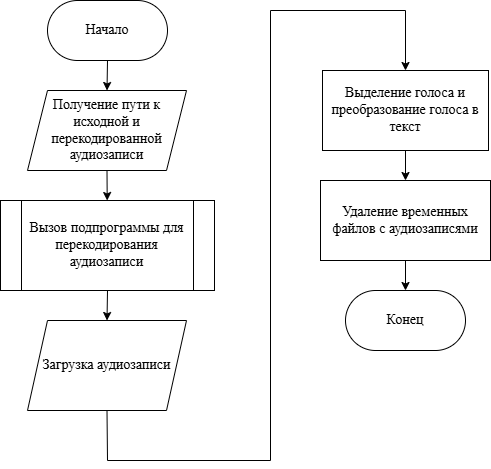
\includegraphics[width=0.6\linewidth]{
        imgs/audiocaptcha/recognize_audiocaptcha.png
    }
    \caption{Блок-схема процесса распознавания Audio CAPTCHA.}
    \label{fig:recognize-audio}
\end{figure}

\section{Автоматизация решения CAPTCHA в формате изображений}

\textbf{Выбор модели нейронной сети для обучения}

CAPTCHA в формате изображений широко используется для защиты ресурсов от 
автоматизированных ботов и может быть реализована несколькими способами. Как 
правило, такие CAPTCHA направлены на проверку способности пользователя 
распознавать и интерпретировать объекты на изображении. Наиболее распространены 
два варианта реализации (оба варианта реализации проиллюстрированы на рис.~
\ref{fig:example}):

\begin{enumerate}
    \item цельное изображение, содержащее несколько объектов, частично размытых 
    или искажённых, при этом изображение разбито на сетку 3×3 или 4×4. 
    Пользователю предлагается выбрать ячейки, содержащие объекты определённого 
    класса (например, автобусы или светофоры);
    \item составное изображение, сформированное из 9 или 12 отдельных фрагментов 
    (изображений), каждый из которых представляет собой независимое изображение 
    -- зачастую низкого качества, с наложением артефактов или шумов. Задача 
    пользователя -- выбрать те изображения, где присутствует нужный объект.
\end{enumerate}

\begin{figure}[!ht]
    \begin{minipage}[h]{0.49\linewidth}
        \center{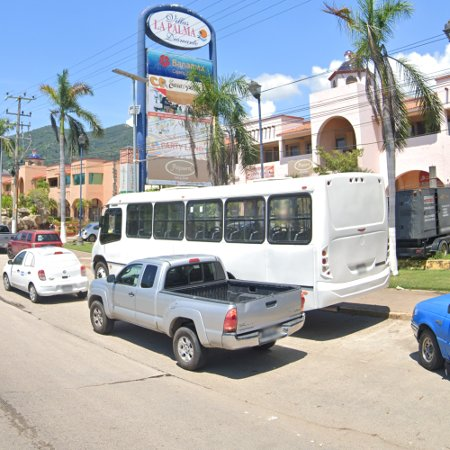
\includegraphics[width=1\linewidth]{imgs/imagecaptcha/6.jpg} \\ 
        а)}
    \end{minipage}
    \hfill
    \begin{minipage}[h]{0.49\linewidth}
        \center{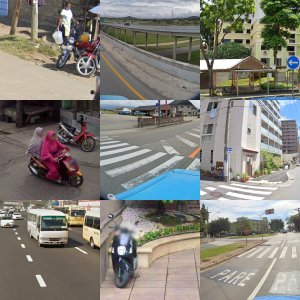
\includegraphics[width=1\linewidth]{imgs/imagecaptcha/8.jpg} \\ 
        б)}
    \end{minipage}
    \caption{Изображения CAPTCHA с размером сетки 3×3: а) -- цельное, б) -- 
    составное.}
    \label{fig:example}
\end{figure}
\vspace{-0.5cm}

Такие CAPTCHA требуют от системы автоматического анализа способности как к 
глобальному восприятию изображения, так и к локальной интерпретации его 
фрагментов. Соответственно, модель, предназначенная для решения данной задачи, 
должна поддерживать:

\begin{enumerate}
    \item классификацию объектов на уровне отдельных изображений (для CAPTCHA, 
    основанных на отдельных картинках в сетке);
    \item локализацию и сегментацию объектов с высокой точностью, чтобы 
    корректно определить границы объектов в пределах ячеек, особенно в случаях, 
    когда объект может частично заходить за границу между ячейками.
\end{enumerate}

Для решения этих задач были рассмотрены следующие современные архитектуры 
нейронных сетей:

\begin{enumerate}
    \item YOLO (You Only Look Once) -- однопроходная модель, объединяющая 
    классификацию и регрессию ограничивающих рамок в одной свёрточной 
    архитектуре. Отличается высокой скоростью и хорошей точностью~
    \cite{redmon2016yolov2, UltralyticsYOLOv8};
    \item Faster R-CNN -- двухступенчатая модель, в которой сначала генерируются 
    области предложений, а затем выполняется классификация и уточнение рамок. 
    Обладает высокой точностью, но уступает в скорости~\cite{ren2015fasterrcnn};
    \item DETR (DEtection TRansformer) -- основана на архитектуре трансформеров, 
    что позволяет эффективно моделировать глобальные взаимосвязи между объектами. 
    Подходит для задач с большим количеством контекстных зависимостей, но требует 
    больше ресурсов для обучения~\cite{carion2020detr}.
\end{enumerate}

Среди этих архитектур было принято решение использовать YOLOv8 по следующим 
причинам:

\begin{enumerate}
    \item высокая производительность: YOLOv8 показывает высокую скорость 
    обработки изображений без значительного ущерба для точности, что критично в 
    условиях, когда необходимо обрабатывать CAPTCHA в реальном времени~
    \cite{bochkovskiy2020yolov4};
    \item гибкость и масштабируемость: модель предоставляет множество 
    предобученных вариантов с различной глубиной и числом параметров (версии n, 
    s, m, l, x), что позволяет использовать как на слабых, так и на 
    производительных устройствах;
    \item широкая поддержка и документация: YOLOv8 имеет активное сообщество, 
    подробную документацию и регулярно обновляется, что значительно упрощает 
    интеграцию и адаптацию модели под пользовательские задачи;
    \item поддержка сегментации: в отличие от более ранних версий, YOLOv8 
    поддерживает не только детекцию, но и сегментацию объектов, что особенно 
    важно для задач, где необходимо точно определить область объекта внутри 
    изображения;
    \item дообучение на пользовательских данных: YOLOv8 позволяет эффективно 
    дообучать модель на собственных датасетах, что особенно важно при работе с 
    CAPTCHA-изображениями, содержащими специфические классы объектов и 
    нестандартные искажения.
\end{enumerate}

Кроме того, модель YOLOv8 была успешно протестирована в задачах, близких по 
структуре к CAPTCHA: детекции дорожных знаков, транспортных средств, пешеходов и 
других объектов в сложных условиях съёмки, что подтверждает её универсальность и 
применимость к рассматриваемой задаче.

Таким образом, YOLOv8 является наиболее сбалансированным выбором, обеспечивающим 
как точную классификацию, так и локализацию объектов в условиях ограниченных 
ресурсов и с возможностью адаптации под специфику визуальных CAPTCHA.

\section{Исследовательский вклад}

\textbf{Тестирование выбранной модели нейронной сети (text captcha)}

Как было установлено в предыдущих разделах, модель последовательного 
преобразования (Seq-to-Seq) продемонстрировала наилучшие результаты среди 
рассмотренных архитектур. Следующим этапом работы являлась оптимизация параметров 
модели, включая веса и коэффициенты регуляризации, с целью ускорения сходимости, 
минимизации риска переобучения и повышения точности распознавания целевых 
последовательностей.

Для проведения экспериментов исходный набор данных, содержащий 100 000 
изображений, был случайным образом перемешан и разделён на три подмножества: 
обучающее, тестовое и валидационное в соотношении 80:10:10. Обучающая выборка 
использовалась непосредственно для обучения модели, валидационная — для контроля 
качества процесса обучения на каждой эпохе, а тестовая — для окончательной 
оценки модели на данных, с которыми она ранее не сталкивалась. В качестве 
основных метрик качества модели использовались функция потерь (loss) и точность 
(accuracy), рассчитываемая для каждого символа последовательности.

В процессе многократного обучения были экспериментально определены оптимальное 
количество эпох и значения гиперпараметров, обеспечивающие эффективное снижение 
функции потерь до приемлемых значений. График сходимости функции потерь 
представлен на рис.~\ref{fig:loss}.

\begin{figure}[H]
    \centering
    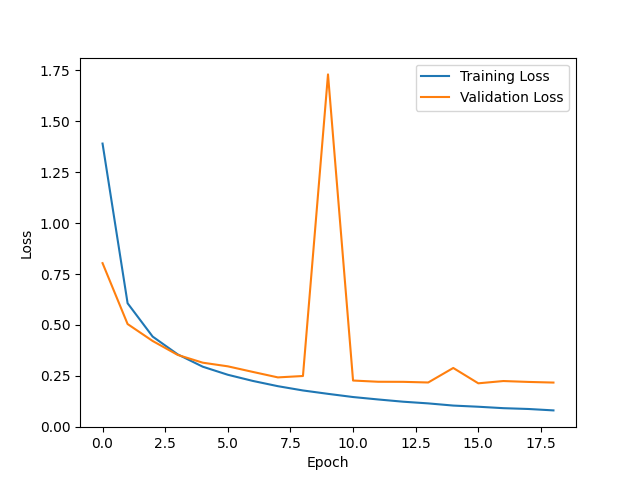
\includegraphics[width=0.8\linewidth]{imgs/textcaptcha/Model_loss.png}
    \caption{График изменения значений функции потерь в процессе обучения.}
    \label{fig:loss}
\end{figure}

Для предотвращения переобучения использовался механизм ранней остановки, согласно 
которому обучение прекращалось при отсутствии уменьшения значения функции потерь 
на валидационной выборке в течение трёх последовательных эпох. В данном 
эксперименте обучение завершилось на 18-й эпохе. На графике видно, что функция 
потерь стабилизировалась после 10 эпохе, поэтому 10 эпоха является балансом между 
точностью распознавания последовательностей и скоростью обучения модели.

Анализ графика сходимости функции потерь показывает наличие резкого увеличения её 
значения на 9-й эпохе, что может быть обусловлено следующими факторами:

\begin{enumerate}
    \item перемешивание данных перед каждой эпохой могло привести к образованию 
    несбалансированной выборки, содержащей значительное число сложных примеров.
    \item динамическое изменение скорости обучения, осуществляемое с помощью 
    механизма регулирования скорости обучения (learning rate scheduler), могло 
    повлиять на изменение функции потерь.
\end{enumerate}

Окончательная точность распознавания отдельных символов составила 0.9263.

После подбора оптимальных значений гиперпараметров модель была сохранена и 
протестирована на валидационной выборке. Точность распознавания 
последовательностей различной длины представлена в таблице~\ref{tab:probability}.

\begin{table}[H]
    \centering
    \caption{Точность предсказаний для последовательностей различной длины.}
    \begin{tabular}{|l|l|}
        \hline
        Длина последовательности & Точность распознавания \\
        \hline
        4 символа & 0.9305 \\
        \hline
        5 символов & 0.7450 \\
        \hline
        6 символов & 0.4575 \\
        \hline
        7 символов & 0.1915 \\
        \hline
    \end{tabular}
    \label{tab:probability}
\end{table}

Также была построена матрица ошибок, позволяющая проанализировать частоту и 
характер ошибок модели при классификации различных классов. Данная матрица 
приведена на рис.~\ref{fig:cm}.

\begin{figure}[H]
    \centering
    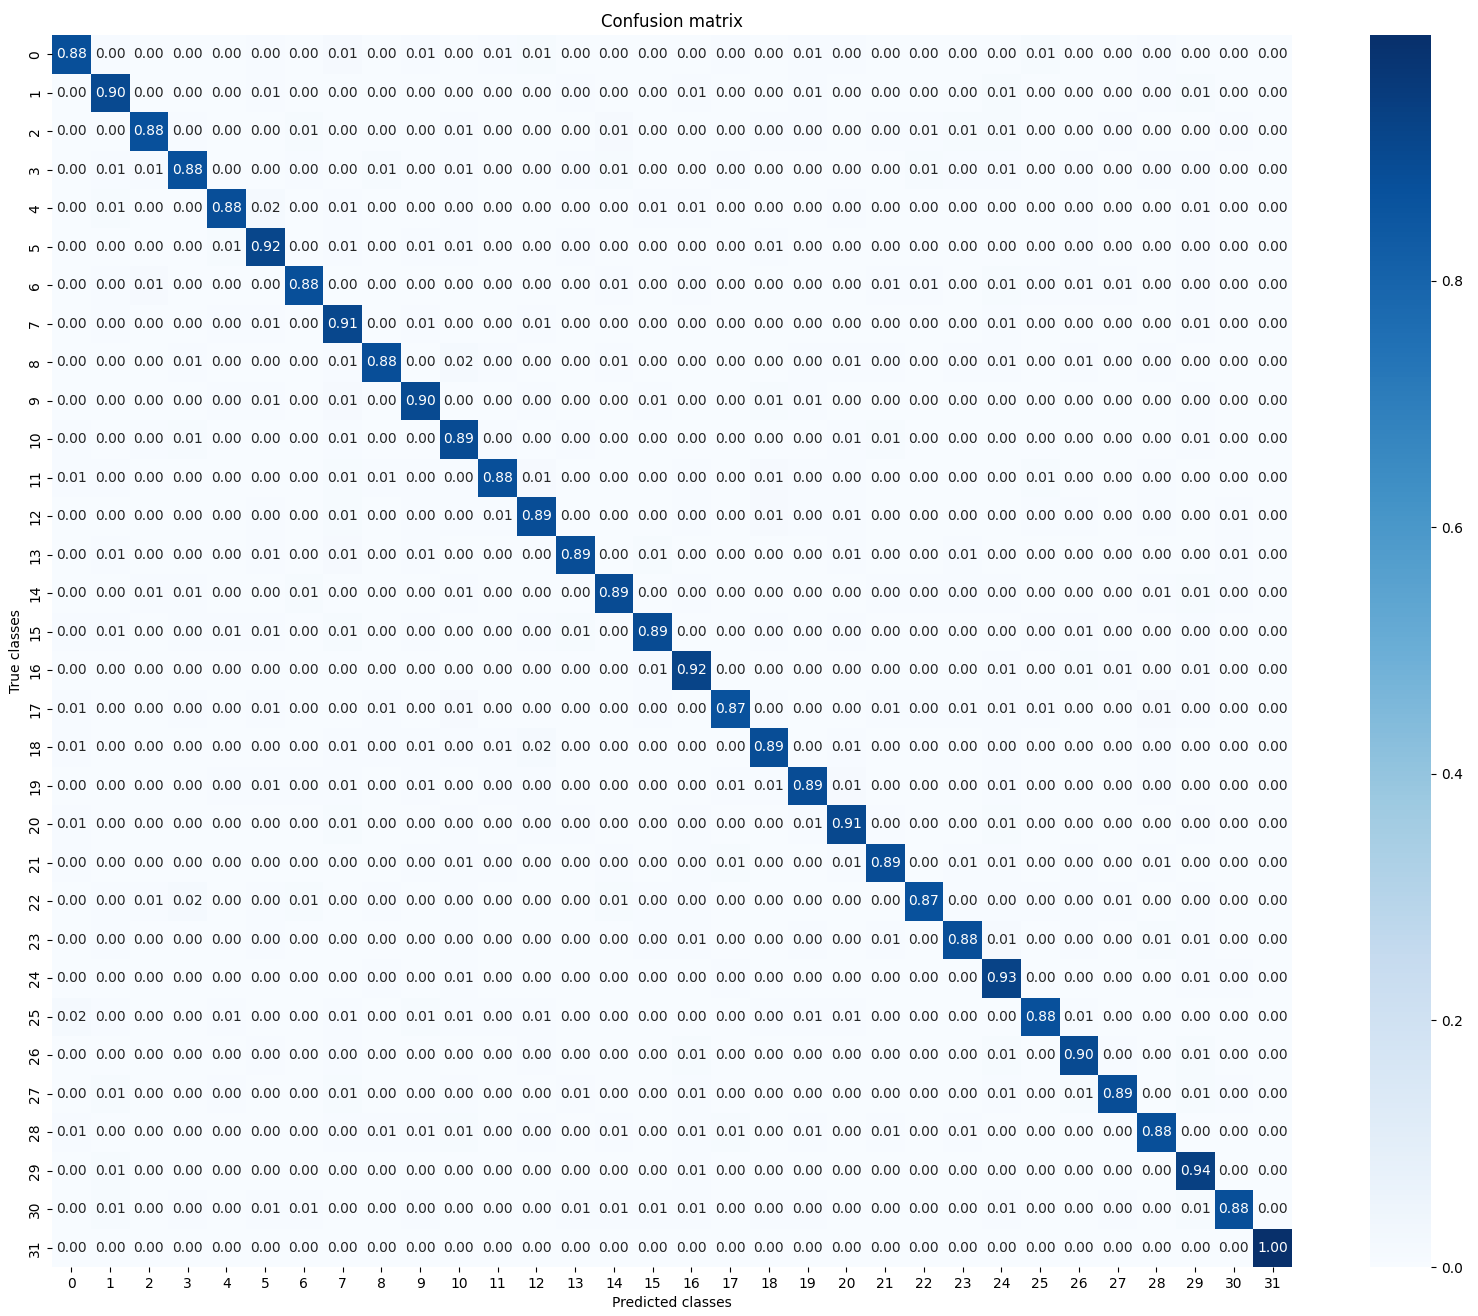
\includegraphics[width=1\linewidth]{imgs/textcaptcha/Confusion_matrix.png}
    \caption{Матрица ошибок для обученной модели.}
    \label{fig:cm}
\end{figure}

Анализ полученных результатов показывает, что точность распознавания 
последовательностей значительной длины остаётся относительно низкой. Это можно 
объяснить высокой зависимостью модели Seq-to-Seq от объёма обучающих данных: для 
эффективного обобщения признаков, извлекаемых из изображений, требуется 
значительное количество примеров. Следовательно, увеличение размера обучающего 
набора данных потенциально может способствовать повышению точности модели, 
однако это также накладывает дополнительные требования к вычислительным ресурсам, 
необходимым для её обучения.

\textbf{Тестирование модели (image captcha)}

После завершения обучения модель была протестирована на реальных CAPTCHA, 
собранных с помощью автоматического парсера, реализованного на базе библиотеки 
Selenium. Тестирование проводилось в автоматическом режиме, имитируя реальные 
действия пользователя в браузере, что позволило оценить работоспособность системы 
в условиях, приближенных к реальной эксплуатации.

Сценарий тестирования предусматривал выполнение следующих шагов:

\begin{enumerate}
    \item автоматический переход к странице с CAPTCHA и активация чекбокса <<Я не 
    робот>>;
    \item извлечение изображения CAPTCHA (включая структуру сетки и текст 
    задания);
    \item определение целевого объекта из текста задания (например, «выберите все 
    изображения с автобусами»);
    \item разбиение изображения CAPTCHA на ячейки (в зависимости от размера сетки 
    -- 3×3 или 4×4);
    \item применение обученной модели для сегментации и классификации каждого 
    изображения или фрагмента;
    \item определение ячеек, содержащих нужный класс, и программная симуляция 
    кликов по ним;
    \item повторная попытка прохождения CAPTCHA в случае, если результат оказался 
    некорректным (что также фиксировалось в логах).
\end{enumerate}

Тестирование было организовано в виде цикла, позволяющего автоматически проходить 
CAPTCHA до тех пор, пока не будет достигнут положительный результат. Это 
позволило зафиксировать частоту ошибок модели и определить случаи, в которых 
требуются дообучение или оптимизация.

Рабочий процесс тестирования и взаимодействия модели с CAPTCHA представлен на 
блок-схеме ниже.

\begin{figure}[H]
    \centering
    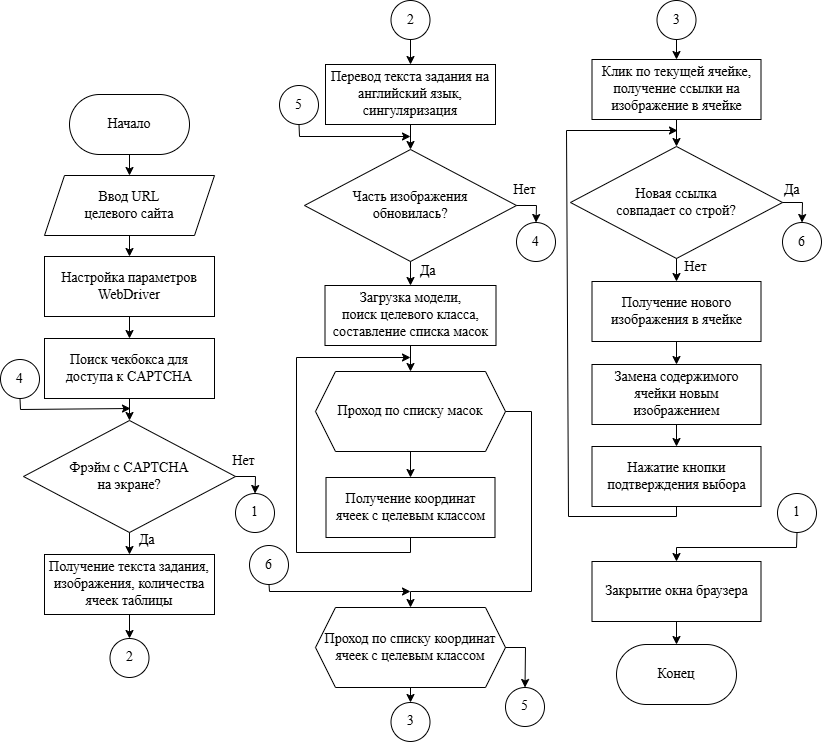
\includegraphics[width=1\textwidth]{imgs/imagecaptcha/solve_captcha_flow.png}
    \caption{Блок-схема процесса прохождения CAPTCHA.}
    \label{fig:solve-captcha}
\end{figure}
\vspace{-0.5cm}

Полученные данные используются для последующего анализа качества модели и 
корректировки процесса обучения. Основное внимание при анализе будет уделено 
типам ошибок, сложности распознаваемых объектов и влиянию качества исходного 
изображения на точность сегментации.

\textbf{Обучение модели}

В качестве основной архитектуры была выбрана модель YOLOv8m-seg, поддерживающая 
сегментацию объектов. Она представляет собой сбалансированное решение между 
качеством распознавания, производительностью и требованиями к аппаратному 
обеспечению. Благодаря своей универсальности, модель подходит как для задач 
классификации, так и для задач детектирования и сегментации, что особенно важно 
при работе с CAPTCHA, содержащими зашумлённые или плохо различимые объекты.

Преимущества YOLOv8m-seg заключаются в следующем:

\begin{enumerate}
    \item наличие встроенной поддержки сегментации объектов, что особенно важно 
    при необходимости выделения фрагментов изображений;
    \item возможность использования предобученных весов, сокращающих время на 
    обучение и повышающих стартовую точность;
    \item высокая скорость инференса по сравнению с другими моделями сегментации 
    (например, Mask R-CNN или DETR);
    \item встроенные средства аугментации (изменения яркости, повороты, 
    масштабирование и пр.);
    \item удобный интерфейс через библиотеку ultralytics, позволяющий быстро 
    запускать обучение, логировать метрики и визуализировать результаты;
    \item полная совместимость с аннотациями в формате YOLO, полученными из CVAT.
\end{enumerate}

Перед запуском обучения структура данных была организована в соответствии с 
требованиями YOLOv8: директории train и val содержали соответствующие изображения 
и файлы разметки, а в .yaml файле конфигурации были указаны пути к выборкам и 
список классов.

Обучение проводилось на 35 эпохах при размере изображений 640×640 пикселей и 
размере батча 8. Использование предобученных весов позволило достичь стабильного 
снижения функции потерь с первых эпох, а встроенные механизмы аугментации 
способствовали улучшению обобщающей способности модели.

Результаты обучения отслеживались по ключевым метрикам (IoU, Precision, Recall, 
Loss), которые визуализировались автоматически. Примеры графиков с результатами 
обучения приведены ниже:

\begin{figure}[H]
    \centering
    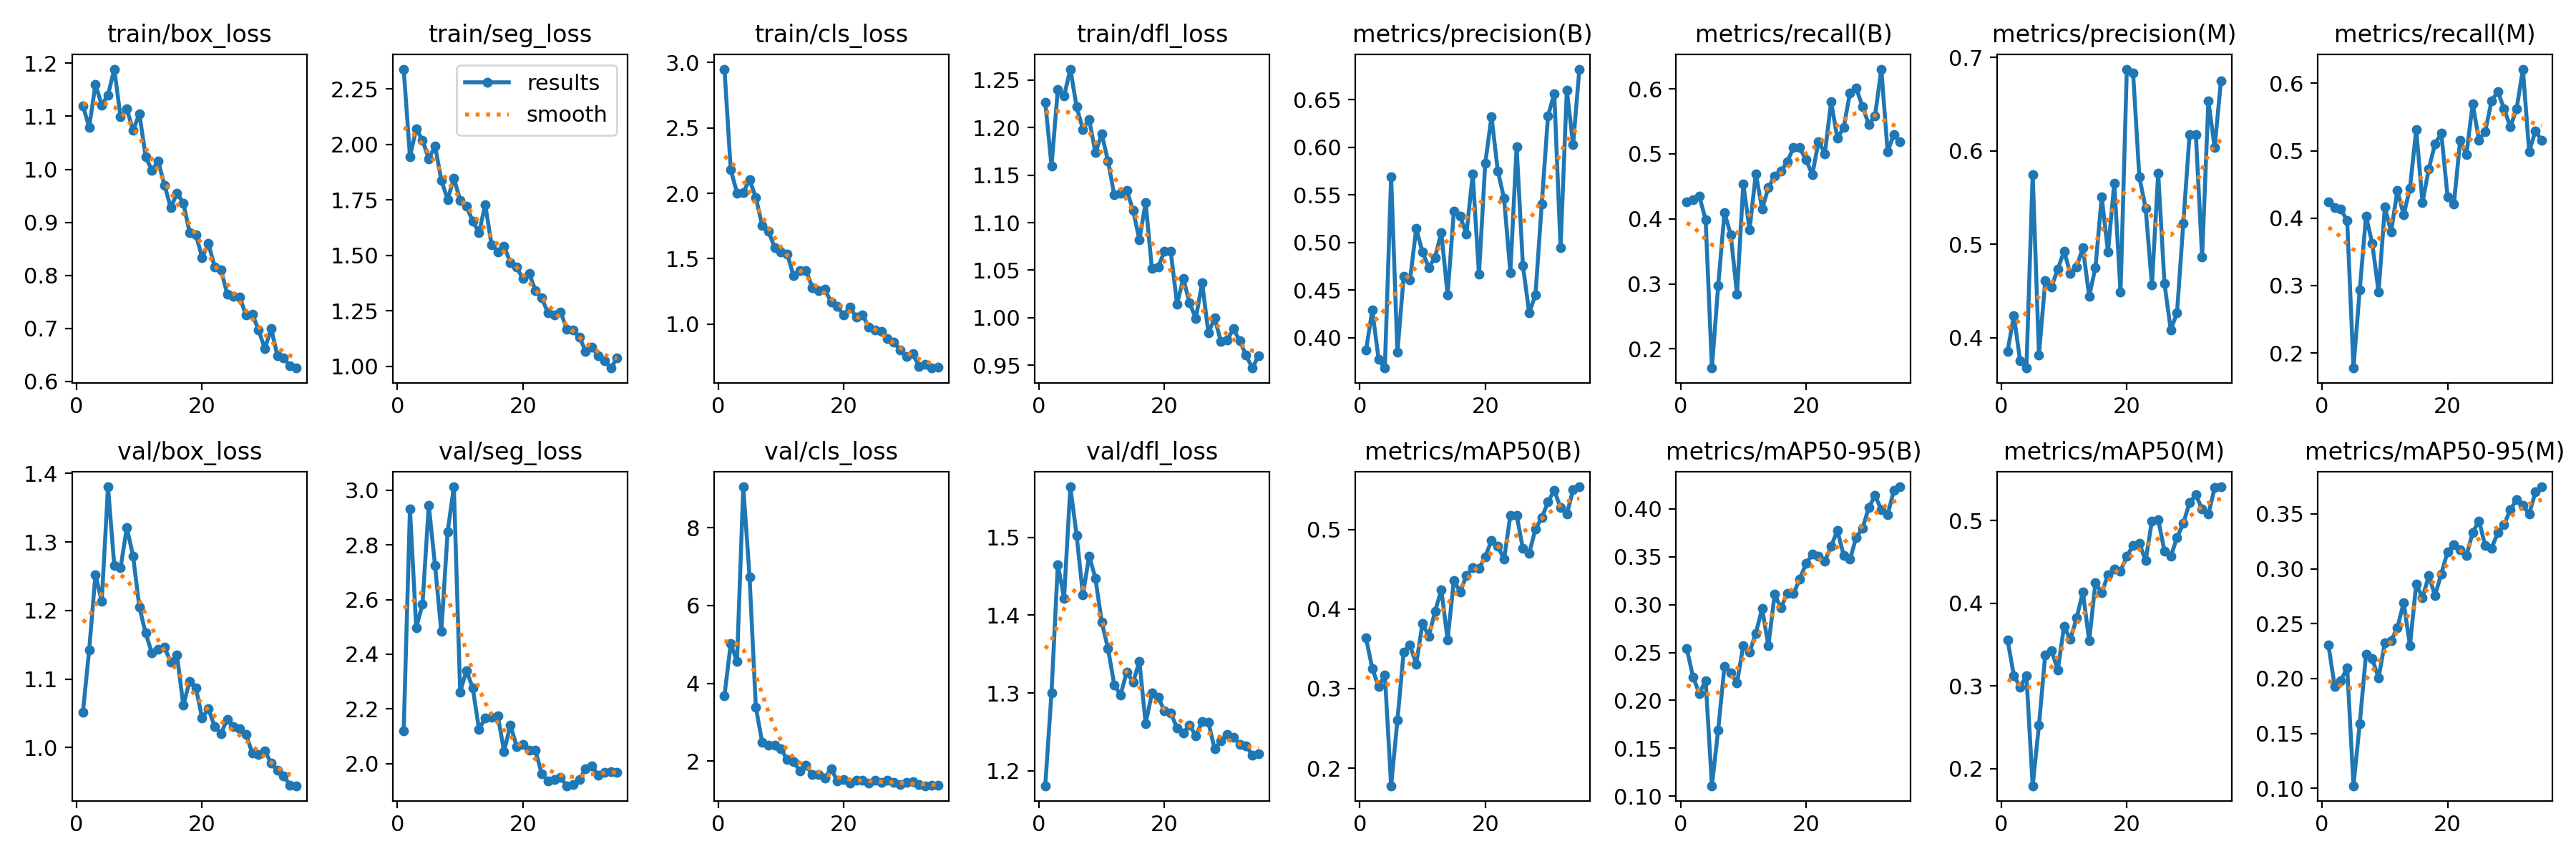
\includegraphics[width=1\linewidth]{imgs/imagecaptcha/results.png}
    \caption{Изменение ключевых метрик в процессе обучения.}
    \label{fig:metrics}
\end{figure}
\vspace{-0.5cm}

Также, была построена нормализованная матрица ошибок для определения точности 
предсказания необходимых классов на валидационной выборке, которая представлена 
на рис.~\ref{fig:confusion}.

\begin{figure}[H]
    \centering
    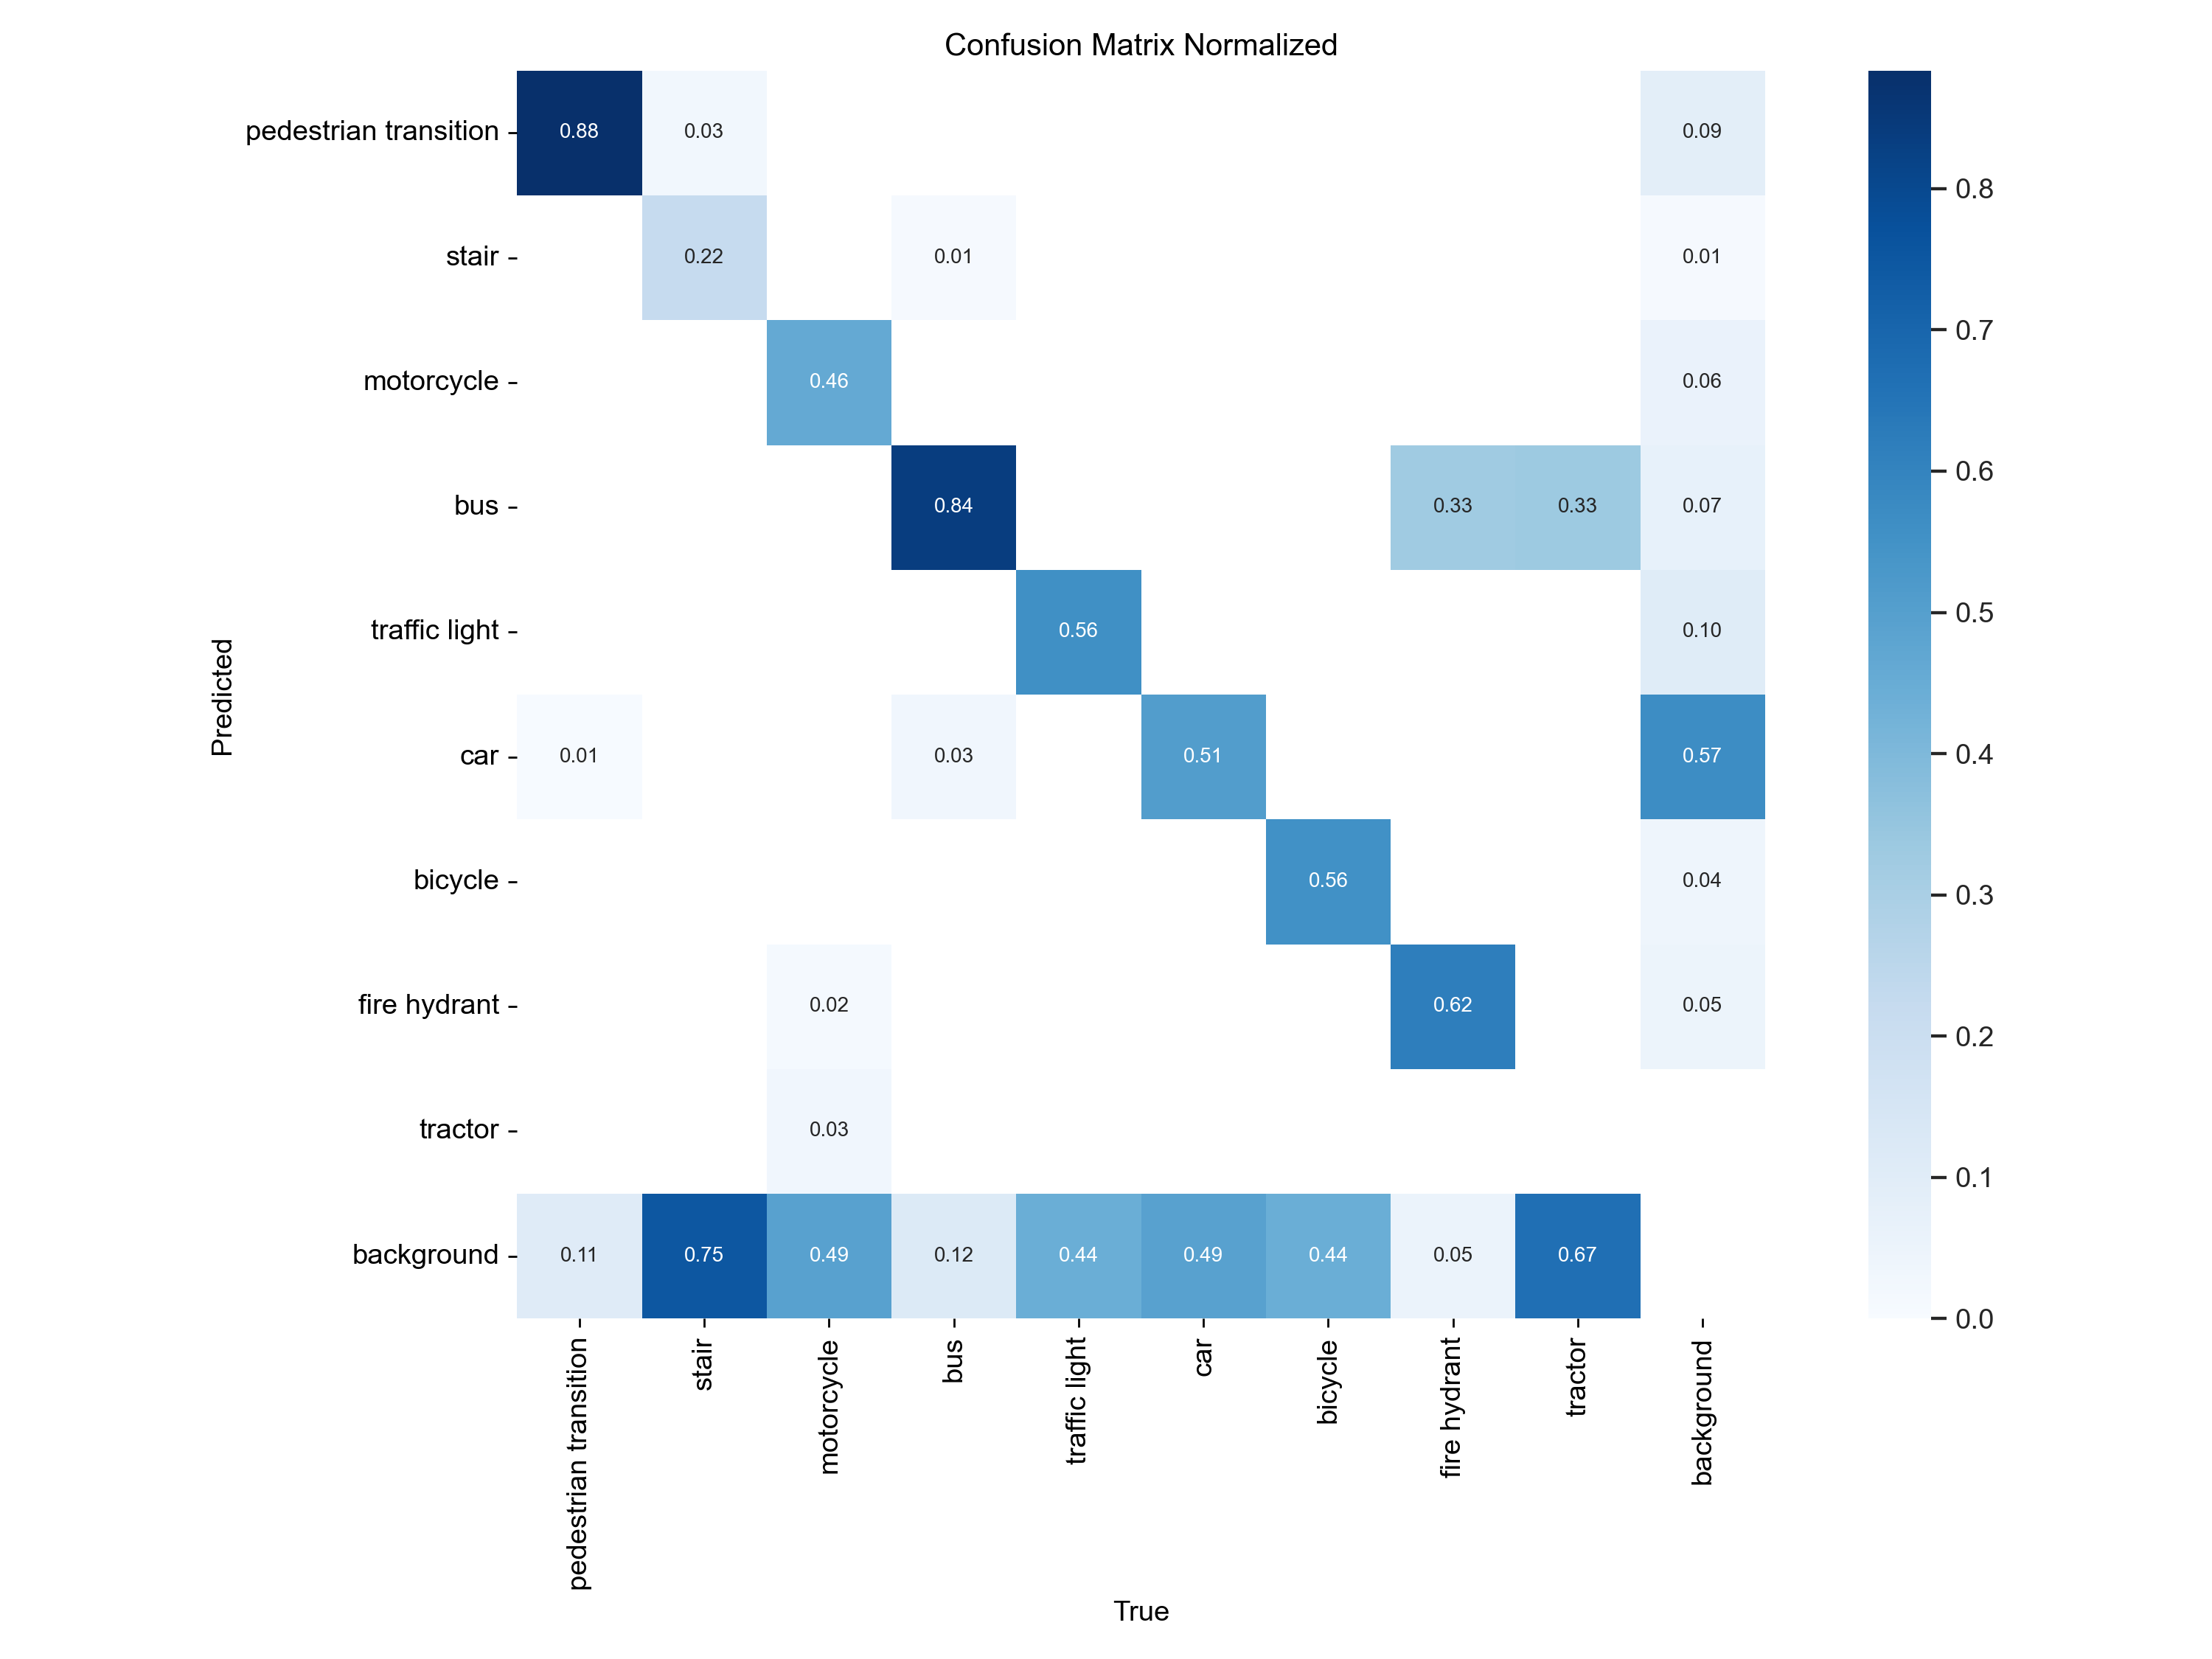
\includegraphics[width=1\linewidth]{
        imgs/imagecaptcha/confusion_matrix_normalized.png
    }
    \caption{Матрица ошибок для изображений валидационной выборки.}
    \label{fig:confusion}
\end{figure}
\vspace{-0.5cm}